\documentclass[11pt, oneside]{article}   	% use "amsart" instead of "article" for AMSLaTeX format
\usepackage{geometry}                		% See geometry.pdf to learn the layout options. There are lots.
\geometry{letterpaper}                   		% ... or a4paper or a5paper or ... 
%\geometry{landscape}                		% Activate for for rotated page geometry
%\usepackage[parfill]{parskip}    		% Activate to begin paragraphs with an empty line rather than an indent
\usepackage{graphicx}				% Use pdf, png, jpg, or eps� with pdflatex; use eps in DVI mode
								% TeX will automatically convert eps --> pdf in pdflatex		
\usepackage{amssymb}

\title{Alberi}
%\author{Fabrizio Demaria}
\date{}							

%
%
% Tutte le immagini sono provvisorie. Le ho inserite per dare un'idea di cosa si potrebbe inserire nel documento finale.
% 
%
%

\begin{document}
\maketitle
\section{Introduzione agli alberi binari}
In teoria dei grafi, un {\em albero} nella sua accezione pi\`u generale corrisponde ad una particolare tipologia di {\em grafo} (non orientato, connesso e aciclico). Per un'esaustiva comprensione dei concetti pi\`u teorici si rimanda dunque al capitolo inerente i grafi. Per gli argomenti trattati in questo capitolo, \`e sufficiente comprendere come pu\`o essere implementata una struttura dati corrispondente ad un {\bf albero binario}. 

Un albero binario \`e composto da {\bf nodi} connessi tra loro mediante certe regole. I nodi della struttura sono i vari oggetti, ognuno contenente un campo chiave e dati satelliti; inoltre i nodi contengono i campi {\em left}, {\em right} e {\em p} che puntano ad altri nodi denominati rispettivamente {\bf figlio sinistro}, {\bf figlio destro} e {\bf padre} del nodo. Ogni nodo di un albero binario pu\`o dunque avere {\em al pi\`u due nodi figli e un unico nodo padre}. Un albero binario presenta un nodo denominato radice ({\em root}), a cui non � connesso alcun nodo padre (nodo 1, nella {\em Figura \ref{fig:Fig_1}}). Infine, nel caso degli alberi binari, non \`e solo importante il numero di figli di un nodo (0, 1 o 2), ma anche la {\em posizione} del figlio: figlio destro o figlio sinistro.

\begin{figure}[h]
\begin{center}
\label{fig:Fig_1}
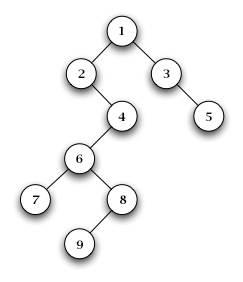
\includegraphics[angle=0,width=0.35\textwidth]{AlberoBinario}
\end{center}
\caption{Esempio di albero binario etichettato con interi}
\end{figure}

Per ci\`o che riguarda il linguaggio di programmazione C, i nodi possono essere implementati mediante {\em struct}, tra i cui campi figurano i puntatori che provvedono alla connessione con il figlio sinistro e il figlio destro (il puntatore al padre solitamente non viene inserito). 
\\

{\em Codice d'esempio:
\\

struct nodo \{

	\ \ \ int key;
	
	\ \ \ struct nodo *left;
	
	\ \ \ struct nodo *right;
	
	\}
}
\\

Questo non \`e l'unico modo con cui pu\`o essere implementato un albero binario in C: anche un semplice array pu\`o essere utilizzato, come vedremo nella sezione del capitolo riguardante gli {\em heap}.

\begin{figure}[h]
\begin{center}
\label{fig:Fig_2}
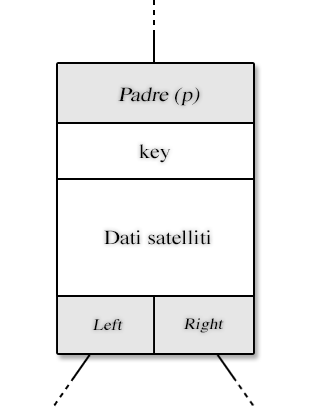
\includegraphics[angle=0,width=0.3\textwidth]{Nodo}
\end{center}
\caption{Possibile struttura di un nodo di albero binario, con le celle grigie puntatori ad altri nodi.}
\end{figure}

Una definizione ricorsiva di albero binario \`e la seguente: un albero binario \`e un insieme finito di nodi e pu\`o essere:
\begin{itemize}
\item
un insieme vuoto, che non contiene nodi, oppure
\item 
\`e composto da tre insiemi disgiunti di nodi: un nodo radice e due alberi binari, rispettivamente {\em sottoalbero sinistro} della radice e {\em sottoalbero destro} della radice.
\end{itemize}

Dato un albero binario $T$ e un suo nodo $x$, un {\em sottoalbero con radice nel nodo x} \`e l'albero indotto dai discendenti del nodo {\em x} e avente come radice {\em x}. Un nodo qualsiasi {\em y} in un cammino unico da {\em r} (radice) a {\em x} \`e detto {\em antenato} di {\em x}. Se {\em y} \`e un antenato di {\em x}, allora {\em x} \`e un {\em discendente} di {\em y}. Se $x \ne y$, allora si parla di {\em antenato proprio} e {\em discendente proprio}. 

Vengono ora elencate ulteriori definizioni:

\begin{itemize}
\item
{\em Foglia}: un nodo senza figli \`e definito come foglia;
\item 
{\em Nodo interno}: un nodo avente almeno un figlio;
\item
{\em Profondit\`a di un nodo}: se la profondit\`a di un nodo \`e $p$ i suoi figli non vuoti hanno profondit\`a $p+1$. La radice $r$ ha profondit\`a 0, i suoi figli sinistro e destro hanno profondit\`a 1, i nipoti profondit\`a 2 e cos\`i via;
\item
{\em Altezza  di un albero}: massima profondit\`a raggiunta dalle sue foglie o, in altri termini, profondit\`a del cammino pi\`u lungo;
\item
{\em Albero binario completo}: albero binario in cui tutte le foglie hanno la stessa profondit\`a e tutti i nodi interni hanno grado 2 (due figli).
\end{itemize}

In un {\bf albero binario completo}, la radice ha 2 figli a profondit\`a 1, ciascuno dei quali ha 2 figli alla profondi\`a 2 e cos\`i via. Quindi, il numero di foglie alla profondit\`a $h$ \`e $2^h$. Il numero totale di nodi risulta essere $2^{(h+1)}-1$. L'altezza di un albero binario completo con $p$ foglie \`e $\log_2(p)$.

%FONTE :http://hbfs.wordpress.com/2009/04/07/compact-tree-storage/
\begin{figure}[h]
\begin{center}
\label{fig:CBT}
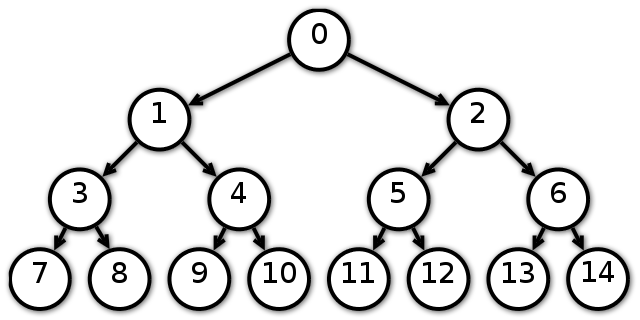
\includegraphics[angle=0,width=0.5\textwidth]{CBT}
\end{center}
\caption{Esempio di un albero binario completo}
\end{figure}


\section{Albero binario di ricerca}

Un {\bf albero binario di ricerca} \`e un albero binario in cui i nodi sono disposti ordinatamente a seconda del valore chiave che li identifica, in modo che valori minori di quelli del nodo di partenza siano memorizzati nei figli a sinistra e i valori pi\`u grandi nei figli a destra.

Sia $x$ un nodo dell'albero binario di ricerca. Se $y$ \`e un nodo nel sottoalbero sinistro di $x$ allora il valore {\em key} di $y$ deve essere minore del valore {\em key} di $x$. Viceversa, se $y$ \`e un nodo nel sottoalbero destro di $x$ allora il valore {\em key} di $y$ deve essere maggiore del valore {\em key} di $x$.
\\

\begin{figure}[h]
\begin{center}
\label{fig:Fig_3}
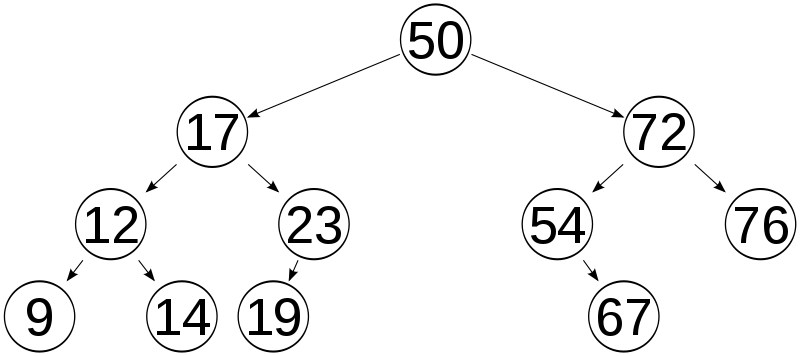
\includegraphics[angle=0,width=0.6\textwidth]{BST}
\end{center}
\caption{Esempio di un albero binario di ricerca}
\end{figure}

Gli alberi di ricerca binari rappresentano una struttura di dati che supporta in modo efficiente le operazioni SEARCH, MINIMUM, MAXIMUM, PREDECESSOR, SUCCESSOR, INSERT, DELETE.
La propriet\`a di ordinamento delle chiavi che contraddistingue un albero binario di ricerca permette di eseguire le operazioni pi\`u comuni, come ad esempio la ricerca di un elemento, con un tempo $O(h)$, dove $h$ \`e l'altezza dell'albero. Per un albero completo con $n$ nodi la complessit\`a risulta essere $\Theta$(lg $n$) nel caso peggiore. Tuttavia, la struttura dell'albero pu\`o degenerare in una catena lineare di $n$ elementi, con conseguente deterioramento delle prestazioni a $\Theta(n)$ nel caso peggiore. 

\subsection{Attraversamento}
\`E possibile elencare ordinatamente tutte le chiavi di un albero binario di ricerca con un semplice algoritmo ricorsivo chiamato {\em attraversamento simmetrico di un albero} (inorder). Tale algoritmo segue la regola per la quale, dato un nodo di un albero binario, prima si visita il figlio sinistro e se tale nodo non esiste si visita il nodo di partenza (stampandone il valore {\em key}) prima di proseguire con la visita del figlio destro (se esiste). Tale regola viene applicata a ogni nodo raggiunto, in modo ricorsivo.
\\

{\em INORDER-VISIT
%IMPLEMENTARE LO PSEUDOCODICE (o il codice C d'esempio)

1

2

3

4
}
\\

%L'immagine provvisoria � stata presa dal seguente link: http://www.technicalypto.com/2010/02/traversals-in-binary-search-tree.html
\begin{figure}[h]
\begin{center}
\label{fig:InOrder}
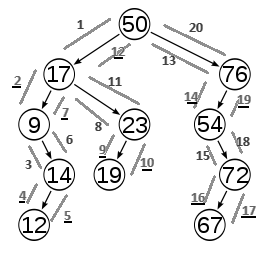
\includegraphics[angle=0,width=0.45\textwidth]{InOrder_copy}
\end{center}
\caption{Attraversamento simmetrico di un albero binario (gli indici sottolineati indicano che la chiave toccata viene aggiunta all'elenco)}
\end{figure}

Con una minima modifica all'algoritmo sopra riportato, \`e possibile definire anche un'{\em attraversamento anticipato di un albero} (preorder), con cui la radice viene elencata prima dei valori dei suoi sottoalberi, e un'{\em attraversamento posticipato di un albero} (postorder), il quale elenca la radice dopo i valori dei suoi sottoalberi. 

Considerando l'albero binario di ricerca della {\em Figura 5} %\ref{fig:InOrder}} <<<usando \ref esce il valore Figura 2.1 invece che Figura 5....
, gli elenchi risultanti dai tre metodi di attraversamento sono i seguenti:

\begin{center}
\begin{tabular}{|c|c|c|}
\hline
{\bf Ordine} 		&		 {\bf Sequenza}	\\
\hline\hline
In-Order		&		\ \ \ \ \ 9, 12, 14, 17, 19, 23, 50, 54, 67, 72, 76\ \ \ \ \ \\
\hline
Pre-Order		&		\ \ \ \ \ 50, 17, 9, 14, 12, 23, 19, 76, 54, 72, 67\ \ \ \ \ \\
\hline
Post-Order	&		\ \ \ \ \ 12, 14, 9,19, 23, 17, 67, 72, 54, 76, 50\ \ \ \ \ \\		
\hline

\end{tabular}
 
\end{center}

\subsection{Ricerca}
L'algoritmo di ricerca per un albero binario di ricerca, dato un puntatore alla radice dell'albero e una chiave $k$, restituisce un puntatore a un nodo con chiave $k$ se esiste, altrimenti restituisce il valore NIL.
\\

{\em SEARCH
%IMPLEMENTARE LO PSEUDOCODICE (o il codice C d'esempio)

1

2

3

4

5
}
\\

La ricerca di un elemento in un albero binario di ricerca \`e basata su di un efficiente algoritmo a carattere ricorsivo.
La procedura inizia la sua ricerca dalla radice e prosegue verso il basso lungo l'albero, quindi il tempo di esecuzione \`e $O(h)$, dove $h$ \`e l'altezza dell'albero.


Per ogni nodo $x$ che viene visitato, si confronta la chiave $k$ con $key[x]$. Se le due chiavi sono uguali la ricerca termina, altrimenti la ricerca prosegue lungo il sottoalbero sinistro se $key$ \`e minore di $key[x]$ o lungo il sottoalbero destro se $key$ \`e maggiore di $key[x]$. Tale processo restituisce il risultato corretto grazie alla propriet\`a fondamentale degli alberi binari di ricerca, per la quale se $k$ \`e minore di $key[x]$, $k$ non pu\`o essere memorizzata nel sottoalbero destro del nodo $x$ (e viceversa).

\subsection{Inserimento}
La procedura di inserimento di un elemento  \`e relativamente semplice e comparabile a quella di ricerca sotto molti aspetti. Ovviamente, \`e sempre necessario inserire un elemento mantenendo valide tutte le propriet\`a strutturali dell'albero binario di ricerca. 
\\

{\em INSERT
%IMPLEMENTARE LO PSEUDOCODICE (o il codice C d'esempio)

1

2

3

4

5

6

7

8

9

10

11

12

13
}
\\

La ricerca della posizione in cui inserire l'elemento parte dalla radice dell'albero e si sposta verso il basso, nei sottoalberi sinistro o destro a seconda dell'esito del confronto tra la chiave dell'elemento visitato e quella dell'elemento da inserire. Un puntatore aggiuntivo mantiene sempre disponibile l'accesso al padre del nodo visitato dal puntatore primario: quando a quest'ultimo viene assegnato il valore NIL \`e stata raggiunta la posizione in cui inserire l'elemento; l'inserimento vero e proprio fa uso del puntatore secondario per l'accesso alla regione di memoria richiesta.

%Inserire figura esplicativa, eventualmente

Analogamente alle altre operazioni elementari con gli alberi di ricerca, la procedura di inserimento viene eseguita in tempo $O(h)$, con $h$ l'altezza dell'albero.
\\

\subsection{Cancellazione}
La cancellazione di un elemento da un albero binario di ricerca \`e un'operazione pi\`u complicata, che varia a seconda che il nodo da cancellare non abbia figli o ne abbia uno o due.

Se il nodo da cancellare $z$ non ha figli ($z$ \`e una foglia dell'albero), \`e sufficiente operare sul padre $p[z]$ per sostituire $z$ con il valore NIL.

Se il nodo $z$ ha un figlio, \`e necessario creare un nuovo collegamento tra il padre e il figlio di $z$ prima di effettuare la cancellazione.

Il caso con due figli collegati a $z$ \`e il pi\`u complicato. E' possibile operare sia sul sottoalbero sinistro del nodo da cancellare che su quello destro. Il primo passo consiste nel trovare l'elemento con chiave maggiore a tutte le altre nel sottoalbero sinistro (l'elemento pi\`u a destra del sottoalbero)  oppure l'elemento con chiave minore nel sottoalbero destro (l'elemento pi\`u a sinistra del sottoalbero). Una volta individuato l'elemento descritto, che indichiamo con $x$, \`e necessario creare un collegamento tra il padre e l'eventuale figlio dell'elemento stesso ($x$ per definizione avr\`a al pi\`u un figlio); successivamente si sovrascrivono la chiave e i dati satelliti dell'elemento $x$ nell'elemento $z$, per poi di procedere alla cancellazione di $x$.

%Inserire il codice (se previsto) ed una eventuale figura comprendente i tre casi di cancellazione dal BST

Nonostante la maggiore complessit\`a di codice, la procedura viene eseguita sempre nel tempo $O(h)$, in un albero di altezza $h$.


%Per il capitolo riguardante gli heap non ho inserito alcun riferimento a codice o pseudocodice.
\section{Heap}
Un {\em heap} (binario) \`e un albero binario con una {\em propriet\`a strutturale} e una {\em proprie\`a funzionale} specifiche: 
\begin{itemize}
\item
{\em Propriet\`a strutturale}: \`e un albero binario {\em quasi completo} (tutti i livelli di profondi\`a sono completi ad eccezione dell'ultimo, che pu\`o essere non completo ma che viene riempito sempre da sinistra a destra).
\item 
{\em Propreit\`a funzionale}: per ogni nodo che non \`e la radice dell'albero, la chiave di tale nodo \`e sempre {\em minore o uguale} alla chiave del padre.
\end{itemize}

Da queste osservazioni sulla struttura di un heap si evince che la chiave con valore massimo tra quelle memorizzate risiede nella radice dell'albero (l'heap \`e del tipo {\em max-heap}). \`E tuttavia possibile imporre che le chiavi dei vari nodi siano sempre {\em maggiori o uguali} delle chiavi dei rispettivi padri, cosicch\'e nella radice dell'albero si trovi la chiave minore (in questo caso si parla di {\em min-heap}).
Gli heap sono alla base dell'algoritmo di ordinamento denominato {\em heapsort}; inoltre la struttura heap realizza un'efficiente coda di priorit\`a.
\\

La struttura dati di un heap prevede dunque un albero binario. Per ci\`o che riguarda l'implementazione, nel caso degli heap si adotta un semplice {\bf array} $A$ avente due attributi: {\em lenght}[{\em A}], che indica la dimensione dell'array, e {\em heap-size}[{\em A}], che indica il numero degli elementi dell'heap memorizzati nell'array (il numero deve essere minore o uguale alla dimensione dell'array).

Per registrare nell'array le informazioni di parentela tra i vari nodi si adottano le seguenti regole: se $i$ \`e l'indice di un nodo, la posizione nell'array in cui si  trova il {\bf figlio sinistro} \`e $2i+1$, quella del {\bf figlio destro} \`e $2i+2$. La radice dell'albero \`e registrata in $A$[$0$].

La {\em Figura 6} %\ref{fig:heap} %problema con i riferimenti una volta che si compila il file tex!!
riassume i concetti descritti fino a questo punto, mostrando un esempio di heap e la relativa implementazione con l'array (nel caso d'esempio la dimensione dell'array coincide con la dimensione dell'heap).

%FONTE: http://scienceblogs.com/goodmath/2008/04/29/implementing-compact-binary-he/
\begin{figure}[h]
\begin{center}
\label{fig:heap}
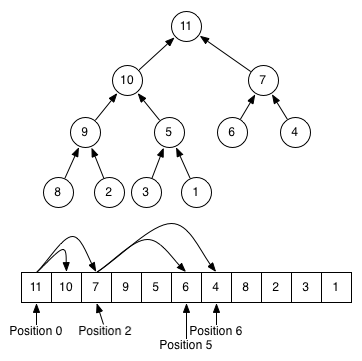
\includegraphics[angle=0,width=0.6\textwidth]{heap}
\end{center}
\caption{Esempio di un heap con relativa implementazione nell'array}
\end{figure}

\subsection{Operazioni sugli heap}
Le operazioni fondamentali eseguite sugli heap richiedono un tempo $O($lg $n)$, con $n$ uguale al numero degli elementi. Tra queste andremo ad analizzare la procedura di inserimento. Successivamente verranno introdotte ulteriori procedure specifiche degli heap spiegando come vengono utilizzate in un algoritmo di ordinamento e in una coda di priorit\`a.

Per la successiva parte del capitolo si assume che l'heap sia del tipo {\bf max-heap} (nella radice dell'albero \`e memorizzata la chiave con il valore massimo).

\subsubsection{Inserimento}
Il primo passo necessario per inserire un elemento in un heap consiste nell'aggiungere una foglia all'albero binario seguendo la {\em propriet\`a strutturale} (riempimento dell'ultimo livello da sinistra a destra). Anche la {\em propriet\`a funzionale} deve essere mantenuta, dunque \`e necessario seguire il cammino dalla foglia fino, al pi\`u, alla radice dell'albero, comparando il valore chiave dei nodi attraversati con quello dell'elemento che si desidera inserire: se necessario si deve far "discendere" i nodi gi\`a memorizzati lungo il ramo di appartenenza fino a quando non viene trovata lo posizione corretta dove inserire il nuovo elemento, tale per cui la chiave del padre risulti maggiore della propria (oppure la posizione corrisponde alla radice dell'albero).

La procedura fondamentale di INSERT, come gi\`a anticipato, risulta avere complessit\`a temporale  $O($lg $n)$. 

%FONTE: http://staff.ustc.edu.cn/~csli/graduate/algorithms/book6/chap07.htm
\begin{figure}[h]
\begin{center}
\label{fig:insert}
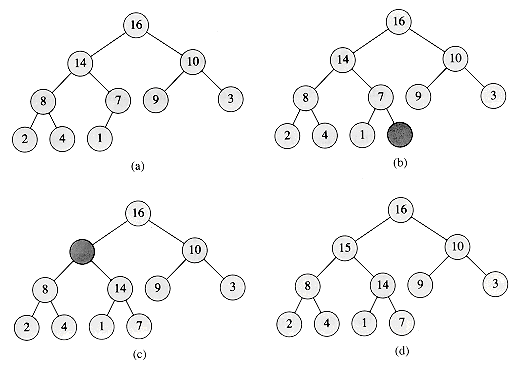
\includegraphics[angle=0,width=0.7\textwidth]{Insert}
\end{center}
\caption{Inserimento dell'elemento 15 nell'heap d'esempio}
\end{figure}


\subsubsection{Heapify}
HEAPIFY \`e un'operazione che riceve come input l'array $A$ e un indice $i$ dell'array. Nel caso in cui $A[i]$ sia pi\`u piccolo dei suoi figli LEFT($i$) o RIGHT($i$), si viola la propriet\`a funzionale degli heap. Supponendo che i sottoalberi con radici LEFT($i$) e RIGHT($i$) siano effettivamente heap, la procedura di HEAPIFY consente al valore $A[i]$ di "scendere" in modo opportuno lungo l'albero: al termine dell'operazione il sottoalbero con radice in $i$ diventa un heap.

Assumendo che LEFT($i$) e RIGHT($i$) siano heap, il primo passo consiste nello scambiare il valore $A[i]$ con il massimo valore tra $A[i]$, LEFT($i$) e RIGHT($i$). Se lo scambio \`e avvenuto con il figlio sinistro si applica ricorsivamente HEAPIFY nel sottoalbero con radice in LEFT($i$), se lo scambio \`e avvenuto con il figlio destro HEAPIFY viene eseguito sul sottoalbero destro. \`E necessario applicare ricorsivamente HEAPIFY sui sottoalberi in quanto a seguito di uno scambio di valori non \`e detto che il sottoalbero interessato mantenga le propriet\`a di un heap (bisogna verificare con il nuovo valore "ereditato" dal padre).
La procedura termina non appena $A[i]$ risulti essere il pi\`u grande tra $A[i]$, LEFT($i$) e RIGHT($i$) (o se si raggiunge una foglia).

HEAPIFY \`e un'operazione con complessit\`a logaritmica: $T$(n)=$O$(lg $n$).

%FONTE: http://www2.hawaii.edu/~suthers/courses/ics311f12/Notes/Topic-09.html
\begin{figure}[h]
\begin{center}
\label{fig:heapify}
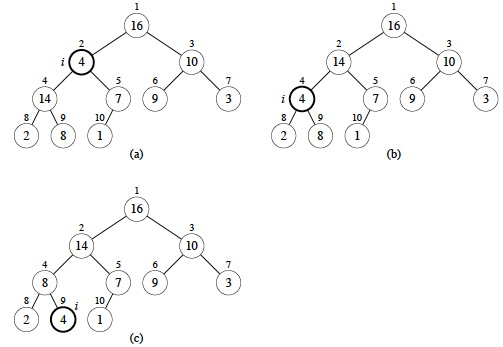
\includegraphics[angle=0,width=0.8\textwidth]{heapify}
\end{center}
\caption{Heapify applicato al nodo 2 dell'heap d'esempio}
\end{figure}

\subsubsection{Build-Heap}
BUILDHEAP \`e la procedura che permette di riposizionare gli elementi memorizzati in un array generico $A$ per convertire $A$ in un heap. Tale procedura consiste nell'applicare ripetutamente HEAPIFY, partendo dal nodo padre della foglia pi\`u a destra per poi proseguire con i rimanenti nodi interni, seguendo a ritroso gli indici dell'array, fino alla radice (indice 0). Come risultato l'array viene convertito in un heap.

BUILDHEAP \`e un'operazione con complessit\`a lineare: $T$(n)=$O$($n$).

%from Cormen
\begin{figure}[h]
\begin{center}
\label{fig:buildh}
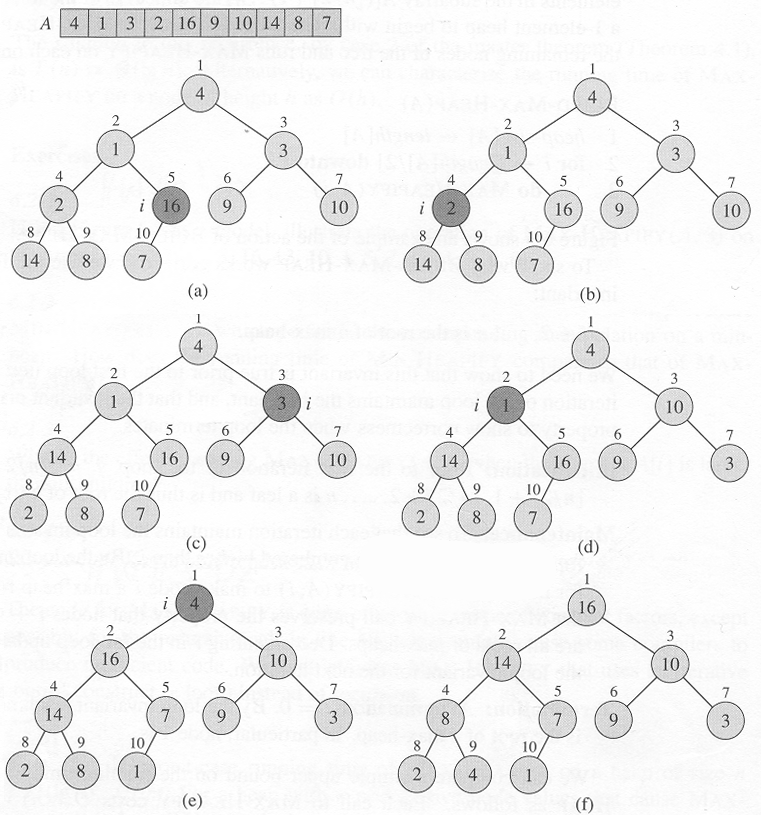
\includegraphics[angle=-0,width=0.80\textwidth]{buildh}
\end{center}
\caption{BUILDHEAP applicato ad un array generico A. Per ogni figura viene applicato HEAPIFY al nodo pi\`u scuro}
\end{figure}

\subsection{Heapsort}
L'algoritmo heapsort \`e un algoritmo di ordinamento efficiente, il cui tempo di esecuzione \`e limitato a $O(n$ lg$n$). Heapsort si basa sulle operazioni eseguibili sugli heap precedentemente descritte.

L'algoritmo ha come input l'array $A$[0,...,($n-1$)] da ordinare. Il primo passo consiste nel convertire tale array in un heap utilizzando BUILDHEAP. Al termine del processo di BUILDHEAP, l'elemento dell'array con valore pi\`u alto \`e memorizzato nella radice dell'albero, cio\`e nella posizione 0 dell'array: si pu\`o dunque spostare tale elemento nella sua posizione finale, scambiandolo con l'ultimo elemento $A[n-1]$. Se ora si riduce di una unit\`a il valore di {\em heap-size}$[A]$, scartando dall'heap il nodo gi\`a posizionato in modo definitivo, si pu\`o notare che i figli della radice restano heap, e solo la nuova radice (ottenuta come risultato del precedente scambio) pu\`o violare le propriet\`a degli heap: per ottenere nuovamente un heap corretto \`e sufficiente applicare HEAPIFY alla radice. Successivamente possiamo essere certi che il nuovo valore massimo dell'heap (il secondo maggiore nell'array) sia memorizzato nella radice, e si procede con un nuovo scambio tra $A[0]$ e $A[n-2]$. Ora si pu\`o ridurre nuovamente il valore di {\em heap-size}$[A]$ e continuare con la medesima procedura, fino a un heap di dimensione 2. Al termine, l'array sar\`a ordinato.

%from Cormen
\begin{figure}[h]
\begin{center}
\label{fig:hs}
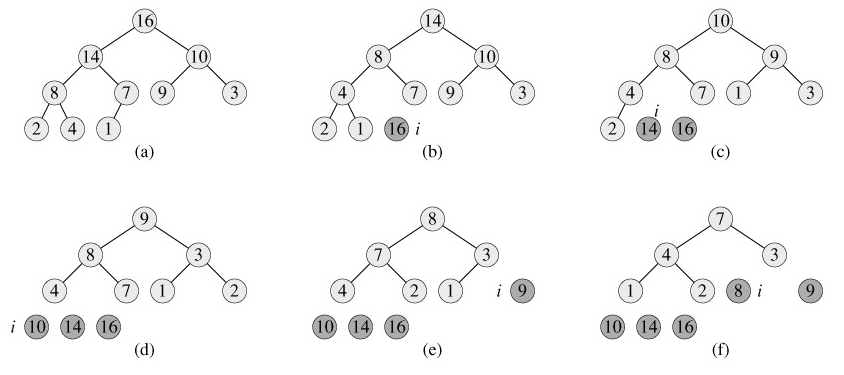
\includegraphics[angle=-0,width=1\textwidth]{hs}
\end{center}
\caption{(a) La struttura iniziale subito dopo BUILDHEAP. (b)-(f) I primi 5 passi dell'algoritmo di ordinamento (la struttura \`e quella subito successiva al processo di HEAPIFY eseguito alla radice). Solo i nodi chiari restano nell'heap, quelli scuri sono ordinati}
\end{figure}

\subsection{Code di priorit\`a}
Una coda di priorit\`a \`e una struttura dati in cui ogni elemento memorizzato \`e associato a una chiave, che ne indica il livello di priorit�\`a; una coda di {\em max-priorit\`a} supporta le seguenti operazioni: 
\begin{itemize}
\item
INSERT: inserisce un elemento nella struttura;
\item
MAXIMUM: restituisce l'elemento con la chiave pi\`u grande;
\item
EXTRACT-MAX: restituisce l'elemento con la chiave pi\`u grande eliminandolo dalla coda di priorit\`a;
\item
INCREASE-KEY: aumenta il valore chiave di un dato elemento;
\end{itemize}

Tale struttura di dati \`e fondamentale in numerose applicazioni, quali la programmazione dei lavori con diversi livelli priorit\`a o la simulazione controllata di eventi. 
%ulteriori approfondimenti possono essere aggiunti sulle applicazioni in cui vengono usate code di priorit�.
\\

Un heap pu\`o implementare un'efficiente coda di priorit\`a. L'operazione MAXIMUM, ad esempio, consiste semplicemente nell'accedere all'elemento radice dell'heap, con costo unitario: $\Theta(1)$. Tutte le altre operazioni sopra elencate, inerenti le code di priorit\`a, hanno un costo pari a $O($lg $n$) nel caso di un'implementazione con heap di $n$ elementi.
%se necessario si possono aggiungere i codici (o pseudocodici) degli algoritmi citati

\end{document}  